%%%%%%%%%%%%%%%%%%%%%%%%%%%%%%%%%%%%%%%%%%%%%%%%%%%%%%%%%%%%%%%%%
% MUW Presentation
% LaTeX Template
% Version 1.0 (27/12/2016)
%
% License:
% CC BY-NC-SA 4.0 (http://creativecommons.org/licenses/by-nc-sa/3.0/)
%
% Created by:
% Nicolas Ballarini, CeMSIIS, Medical University of Vienna
% nicoballarini@gmail.com
% http://statistics.msi.meduniwien.ac.at/
%
% Customized for UAH by:
% David F. Barrero, Departamento de Automática, UAH
%%%%%%%%%%%%%%%%%%%%%%%%%%%%%%%%%%%%%%%%%%%%%%%%%%%%%%%%%%%%%%%%%

\documentclass[10pt,compress]{beamer} % Change 10pt to make fonts of a different size
\mode<presentation>

\usepackage[spanish]{babel}
\usepackage{fontspec}
\usepackage{tikz}
\usepackage{etoolbox}
\usepackage{xcolor}
\usepackage{xstring}
\usepackage{listings}
\usepackage{multicol}
\usepackage{tabularx}
\usepackage{tikz}
\usetikzlibrary{matrix,chains,positioning,decorations.pathreplacing,arrows,shapes}

\usetheme{UAH}
\usecolortheme{UAH}
\setbeamertemplate{navigation symbols}{} 
\setbeamertemplate{caption}[numbered]

%%%%%%%%%%%%%%%%%%%%%%%%%%%%%%%%%%%%%%%%%%%%%%%%%%%%%%%%%%%%%%%%%
%% Presentation Info
\title[NumPy]{NumPy}
\author{\asignatura\\\carrera}
\institute{}
\date{Departamento de Automática}
%%%%%%%%%%%%%%%%%%%%%%%%%%%%%%%%%%%%%%%%%%%%%%%%%%%%%%%%%%%%%%%%%


%%%%%%%%%%%%%%%%%%%%%%%%%%%%%%%%%%%%%%%%%%%%%%%%%%%%%%%%%%%%%%%%%
%% Descomentar para habilitar barra de navegación superior
\setNavigation
%%%%%%%%%%%%%%%%%%%%%%%%%%%%%%%%%%%%%%%%%%%%%%%%%%%%%%%%%%%%%%%%%

%%%%%%%%%%%%%%%%%%%%%%%%%%%%%%%%%%%%%%%%%%%%%%%%%%%%%%%%%%%%%%%%%
%% Configuración de logotipos en portada
%% Opacidad de los logotipos
\newcommand{\opacidad}{1}
%% Descomentar para habilitar logotipo en pié de página de portada
\renewcommand{\logoUno}{Images/isg.png}
%% Descomentar para habilitar logotipo en pié de página de portada
%\renewcommand{\logoDos}{Images/CCLogo.png}
%% Descomentar para habilitar logotipo en pié de página de portada
%\renewcommand{\logoTres}{Images/ALogo.png}
%% Descomentar para habilitar logotipo en pié de página de portada
%\renewcommand{\logoCuatro}{Images/ELogo.png}
%%%%%%%%%%%%%%%%%%%%%%%%%%%%%%%%%%%%%%%%%%%%%%%%%%%%%%%%%%%%%%%%%

%%%%%%%%%%%%%%%%%%%%%%%%%%%%%%%%%%%%%%%%%%%%%%%%%%%%%%%%%%%%%%%%%
%% FOOTLINE
%% Comment/Uncomment the following blocks to modify the footline
%% content in the body slides. 


%% Option A: Title and institute
\footlineA
%% Option B: Author and institute
%\footlineB
%% Option C: Title, Author and institute
%\footlineC
%%%%%%%%%%%%%%%%%%%%%%%%%%%%%%%%%%%%%%%%%%%%%%%%%%%%%%%%%%%%%%%%%

\begin{document}

%%%%%%%%%%%%%%%%%%%%%%%%%%%%%%%%%%%%%%%%%%%%%%%%%%%%%%%%%%%%%%%%%
% Use this block for a blue title slide with modified footline
{\titlepageBlue
    \begin{frame}
        \titlepage
    \end{frame}
}

\institute{\asignatura}

\begin{frame}[plain]{}
	\begin{block}{Objectives}
		\begin{enumerate}
		\item Understand the limitations of plain Python in scientific computation
		\item Introduce NumPy
		\item Fluent array manipulation with Numpy
		\end{enumerate}
	\end{block}

   \begin{block}{Bibliography}
       Jake VanderPlas. \textit{Python Data Science Handbook}. Chapter 2. O'Reilly. \href{https://jakevdp.github.io/PythonDataScienceHandbook/}{(Link)}.
   \end{block}

\end{frame}

{
\disableNavigation{white}
\begin{frame}[shrink]{Table of Contents}
 \frametitle{Table of Contents}
 \begin{multicols}{2}
 \tableofcontents
 \end{multicols}
  % You might wish to add the option [pausesections]
\end{frame}
}

\section{Introduction}
\subsection{Understanding Data Types in Python}

\begin{frame}{Introduction}{Understanding Data Types in Python (I)}
    %Python supports matrices by default
    %\begin{itemize}
    %    \item Why do we need additional support?
	%\end{itemize}

    \begin{columns}
 	   \column{0.5\textwidth}
			
			\begin{block}{\footnotesize{Static typing}}
			\vspace{-0.2cm} 
				\lstinputlisting[basicstyle=\ttfamily\scriptsize,language=C]{code/static.c}
			\vspace{-0.2cm} 
			\end{block}

			\begin{itemize}
				\item Data types must be declared
				\item Data types cannot change
				\item Error detection in compilation
				\item Variables names are, basicly, labels
			\end{itemize}
			
 	   \column{0.5\textwidth}
			\begin{block}{\footnotesize{Dynamic typing}}
			\vspace{-0.2cm} 
				\lstinputlisting[basicstyle=\ttfamily\scriptsize]{code/dynamic.py}
			\vspace{-0.2cm} 
			\end{block}

			\begin{itemize}
				\item Data types are not declared
				\item Data types can change
				\item Error detection in run-time
				\item Variables are complex data structures (even for simple types)
			\end{itemize}
	\end{columns}
\end{frame}

\begin{frame}{Introduction}{Understanding Data Types in Python (II)}
    %Python supports matrices by default
    %\begin{itemize}
    %    \item Why do we need additional support?
	%\end{itemize}

	Dynamic typing must be implemented somewhere ...

    \begin{columns}
 	   \column{0.5\textwidth}
			\begin{block}{\footnotesize{Python 3.4 source code}}
			\vspace{-0.2cm} 
				\lstinputlisting[basicstyle=\ttfamily\scriptsize, language=C]{code/long.c}
			\vspace{-0.2cm} 
			\end{block}

 	   \column{0.5\textwidth}
			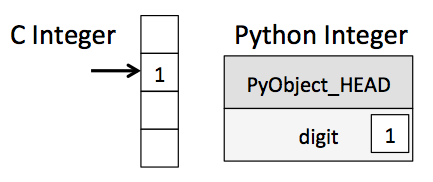
\includegraphics[width=\textwidth]{figs/cint_vs_pyint.png}	
	\end{columns}

\end{frame}

\begin{frame}[fragile]{Introduction}{Understanding Data Types in Python (III)}
	\begin{columns}
 	   \column{0.5\textwidth}
			A Python list may contain different types

 	   \column{0.5\textwidth}
	   \begin{exampleblock}{}
			\vspace{-0.2cm} 
			\lstinputlisting[basicstyle=\ttfamily\scriptsize]{code/lists.txt}
			\vspace{-0.2cm} 
		\end{exampleblock}
	\end{columns}

	\bigskip

	\centering 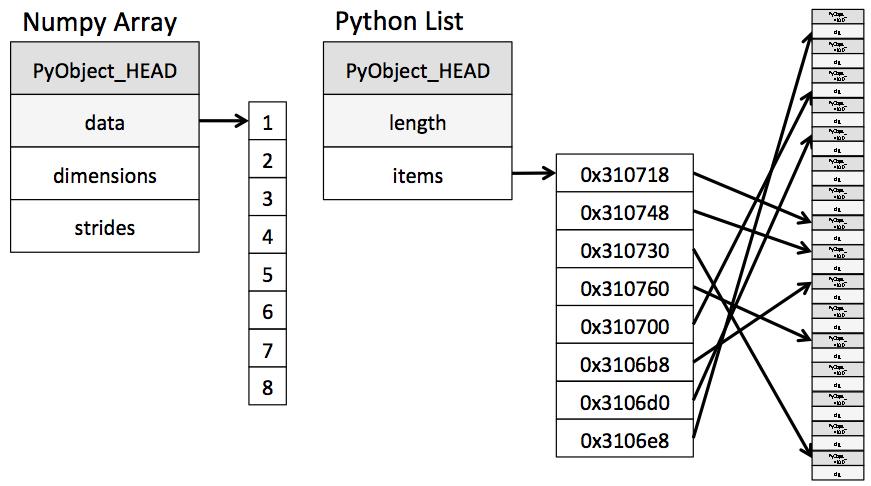
\includegraphics[width=0.8\textwidth]{figs/array_vs_list.png}	
\end{frame}

\begin{frame}[fragile]{Introduction}{Understanding Data Types in Python (IV)}
	Standard Python data types are powerful and flexible
	\begin{itemize}
		\item Flexibility has a price: Reduced performance
		\item Not an big issue in generic programming
		\item A big issue in scientific programming
		\item We require efficient data manipulation mechanisms: NumPy
	\end{itemize}
	NumPy: Python package for numeric computation
	\begin{itemize}
		\item Efficient array implementation
		\item Fast mathematical functions
		\item Random numbers generation
		\item Static data types: Less flexibility
	\end{itemize}
	Most Python modules for AI/ML depend on NumPy, in particular
	\begin{itemize}
		\item Pandas (dataframes), Scikit-learn (ML), Seaborn (data visualization)
	\end{itemize}
\end{frame}

\subsection{NumPy}

\begin{frame}[fragile]{Introduction}{NumPy}
	\begin{columns}
 	   \column{0.6\textwidth}
		NumPy must be imported in order to be available
		\begin{itemize}
			%\item By convention, \texttt{import numpy as np}
			\item Remember, you can use \texttt{np?} or \texttt{np.<TAB>}
		\end{itemize}

		The main component of NumPy is \alert{ndarray}
		\begin{itemize}
			\item Python object
			\item Efficient matrix representation
			\item Homogeneus elements
		\end{itemize}

 	   \column{0.4\textwidth}
		\begin{block}{\footnotesize{Convention}}
		\vspace{-0.2cm} 
			\begin{lstlisting}
			import numpy as np
			\end{lstlisting}
		\vspace{-0.2cm} 
		\end{block}

		\begin{exampleblock}{}
		\vspace{-0.2cm} 
			\begin{lstlisting}
			In [1]: array = np.array([1,2,3])
			In [2]: array
			Out[1]: array([1, 2, 3])
			In [3]: array = np.array([[1,2],[3,4]])
			\end{lstlisting}
		\vspace{-0.2cm} 
		\end{exampleblock}
	\end{columns}
\end{frame}

\section{Matrix creation and manipulation}

\subsection{Matrix creation}
\begin{frame}[fragile]{Matrix creation and manipulation}{Matrix creation}
	NumPy functions for array creation from lists
	\begin{itemize}
		\item Lists must contain the same type, NumPy will upcast if needed
		\item \texttt{np.array([1, 4, 2, 5, 3])}
		\item \texttt{np.array([1, 2, 3, 4], dtype='float32')}: Explicit data type
		\item \texttt{np.array([3.14, 4, 2, 3])}: Upcast
	\end{itemize}
	NumPy functions for array creation from scratch
	\begin{itemize}
		\item \texttt{np.zeros(10, dtype=int)}: All zeros
		\item \texttt{np.ones((3, 5), dtype=float)}: All ones
		\item \texttt{np.full((3, 5), 3.14)}: Fill matrix
		\item \texttt{np.arange(0, 20, 2)}: Similar to Python's range()
		\item \texttt{np.linspace(0, 1, 5)}: Evenly spaced numbers
		\item \texttt{np.random.random((3, 3))}: Random numbers
		\item \texttt{np.random.normal(0, 1, (3, 3))}: Random normal numbers
		\item \texttt{np.random.randint(0, 10, (3, 3))}: Random integers
		\item \texttt{np.eye(3)}: Identity matrix
		\item \texttt{np.empty(3)}: Empty matrix
	\end{itemize}
\end{frame}

\subsection{NumPy data types}
\begin{frame}[fragile]{Matrix creation and manipulation}{NumPy data types}
	\begin{columns}
 	   \column{0.4\textwidth}
	   Python is implemented in C
	   \begin{itemize}
	   	\item Data types in NumPy are based on those in C
	   \end{itemize}
	   Two styles to declare types
	   \begin{itemize}
	   	\item String:\\ \texttt{np.zeros(10, dtype='int16')}
		\item NumPy object: \texttt{np.zeros(10, dtype=np.int16)}
	   \end{itemize}

 	   \column{0.6\textwidth}
	\footnotesize{
    \begin{tabular}{ll}\hline
       \textsc{Data type} &  \textsc{Description}\\ \hline
	   \texttt{bool\_} & Boolean (True or False) stored as a byte  \\
	   \texttt{int\_} & Default integer type  \\
	   \texttt{intc} & Identical to C  \\
	   \texttt{intp} & Integer used for indexing  \\
	   \texttt{int8} & Byte  \\
	   \texttt{int16} & Integer  \\
	   \texttt{int32} & Integer  \\
	   \texttt{int64} & Integer  \\
	   \texttt{uint8} & Unsigned integer  \\
	   \texttt{uint16} & Unsigned integer  \\
	   \texttt{uint32} & Unsigned integer  \\
	   \texttt{uint64} & Unsigned integer  \\
	   \texttt{float\_} & Shorthand for float64  \\
	   \texttt{float16} & Half precision float  \\
	   \texttt{float32} & Single precision float  \\
	   \texttt{float64} & Double precision float  \\
	   \texttt{complex\_} & Shorthand for complex128  \\
	   \texttt{complex64} & Complex number  \\
	   \texttt{complex128} & Complex number  \\\hline
    \end{tabular}
	}
	\end{columns}
\end{frame}

\subsection{NumPy array attributes}
\begin{frame}[fragile]{Matrix creation and manipulation}{NumPy array attributes}
	\begin{columns}
 	   \column{0.5\textwidth}
		Ndarray objects expose several attributes
		\begin{itemize}
			\item \texttt{ndim}: Dimensions
			\item \texttt{shape}: Size of each dimension
			\item \texttt{size}: Number of elements
			\item \texttt{dtype}: Data type
			\item \texttt{itemsize}: Size of each element (in bytes)
			\item \texttt{nbytes}: Size of the array (in bytes)
		\end{itemize}

 	   \column{0.5\textwidth}
		\begin{exampleblock}{}
		\vspace{-0.2cm} 
			\begin{lstlisting}
x = np.random.randint(10, size=(3, 4))
print("x ndim: ", x.ndim)
print("x shape:", x.shape)
print("x size: ", x.size)
print("dtype:", x.dtype)
print("itemsize:", x.itemsize)
print("nbytes:", x.nbytes)
			\end{lstlisting}
		\vspace{-0.2cm} 
		\end{exampleblock}
	\end{columns}
\end{frame}

\subsection{Accessing single elements}
\begin{frame}[fragile]{Matrix creation and manipulation}{Accessing single elements}
	\begin{columns}
 	   \column{0.5\textwidth}
		Unidimensional array
		\begin{itemize}
			\item \texttt{array[index]}
		\end{itemize}
		Unidimensional array from the end
		\begin{itemize}
			\item \texttt{array[-index]}
		\end{itemize}
		Multidimensional array
		\begin{itemize}
			\item \texttt{array[row,column]}
		\end{itemize}

 	   \column{0.5\textwidth}
		\begin{exampleblock}{}
		\vspace{-0.2cm} 
			\begin{lstlisting}
x = np.array([5, 0, 3, 3, 7, 9])
x[0] # 5
x[4] # 7
x[-1] # 9
x[-2] # 7
x = np.array([[3, 5, 2, 4],
    [7, 6, 8, 8],
    [1, 6, 7, 7]])
x2[2, 0] # 1 
x2[2, -1] # 7
			\end{lstlisting}
		\vspace{-0.2cm} 
		\end{exampleblock}
	\end{columns}

	\smallskip

	\begin{columns}
 	   \column{0.6\textwidth}
		\begin{alertblock}{Warning}
			Ndarray has fixed types, values can be truncaded without warning. Big source of problems!
		\end{alertblock}
	\end{columns}

\end{frame}

\subsection{Accessing subarrays}
\begin{frame}[fragile]{Matrix creation and manipulation}{Accessing subarrays}
	\begin{columns}
 	   \column{0.5\textwidth}
		Slice notation can be used with ndarray
		\begin{itemize}
			\item \texttt{x[start:stop:step]}
		\end{itemize}
		Default values
		\begin{itemize}
			\item Start = 0
			\item Stop = Size of dimension
			\item Step = 1
		\end{itemize}
		Step may take a negative value
		\begin{itemize}
			\item Reverse order
		\end{itemize}
		These operations return a view 
		\begin{itemize}
			\item Use \texttt{copy()} to get a copy
		\end{itemize}

 	   \column{0.5\textwidth}
		\begin{exampleblock}{\footnotesize{Unidimensional array}}
		\vspace{-0.2cm} 
			\begin{lstlisting}
x[:5]   # first five elements
x[5:]   # elements after index 5
x[4:7]  # middle sub-array
x[::2]  # every other element
x[1::2] # every other element, starting at index 1
x[::-1] # all elements, reversed
			\end{lstlisting}
		\vspace{-0.2cm} 
		\end{exampleblock}

		\begin{exampleblock}{\footnotesize{Multidimensional a  rray}}
		\vspace{-0.2cm} 
			\begin{lstlisting}
x[:2, :3]  # 2 rows, 3 columns
x[:3, ::2] # all rows, every other column
x[::-1, ::-1]
			\end{lstlisting}
		\vspace{-0.2cm} 
		\end{exampleblock}
	\end{columns}
\end{frame}

\subsection{Reshaping of arrays}
\begin{frame}[fragile]{Matrix creation and manipulation}{Reshaping of arrays}
	\begin{columns}
 	   \column{0.5\textwidth}
		Reshaping arrays is a very common task
		\begin{itemize}
			\item Change data number of dimensions
			% Ejemplo imagen en red neuronal
		\end{itemize}
		Important ndarray method: \texttt{reshape()}
		\begin{itemize}
			\item Changes the dimensions of an array
			\item Sizes must match
		\end{itemize}

 	   \column{0.5\textwidth}
		\begin{exampleblock}{\footnotesize{General reshaping}}
		\vspace{-0.2cm} 
			\begin{lstlisting}
In [1]: x=np.array([1, 2, 3, 4])
In [2]: x.reshape((2,2))
Out[1]: 
array([[1, 2],
       [3, 4]])
			\end{lstlisting}
		\vspace{-0.2cm} 
		\end{exampleblock}
	\end{columns}

	\begin{columns}
	   \column{0.5\textwidth}
		Conversion of 1-D arrays into column or row matrices
		\begin{itemize}
			\item Using method \texttt{reshape()}
			\item Using the keyword \alert{np.newaxis}
		\end{itemize}

 	   \column{0.5\textwidth}
		\begin{exampleblock}{\footnotesize{1-D to row}}
		\vspace{-0.2cm} 
			\begin{lstlisting}
x = np.array([1, 2, 3])
x.reshape((1, 3))
x[np.newaxis, :]
			\end{lstlisting}
		\vspace{-0.2cm} 
		\end{exampleblock}

		\begin{exampleblock}{\footnotesize{1-D to column}}
		\vspace{-0.2cm} 
			\begin{lstlisting}
x.reshape((3, 1))
x[:, np.newaxis]
			\end{lstlisting}
		\vspace{-0.2cm} 
		\end{exampleblock}
	\end{columns}
\end{frame}

\subsection{Concatenation of arrays}
\begin{frame}[fragile]{Matrix creation and manipulation}{Concatenation of arrays}
	\begin{columns}
 	   \column{0.4\textwidth}
		Three methods to join arrays
		\begin{itemize}
			\item \texttt{np.concatenate()}
			\item \texttt{np.vstack()}
			\item \texttt{np.hstack()}
		\end{itemize}

 	   \column{0.6\textwidth}
		\begin{exampleblock}{\footnotesize{np.concatenate()}}
		\vspace{-0.2cm} 
			\begin{lstlisting}
In [1]: x = np.array([1, 2, 3])
In [2]: y = np.array([3, 2, 1])
In [3]: np.concatenate([x, y])
Out[1]: array([1, 2, 3, 3, 2, 1])
			\end{lstlisting}
		\vspace{-0.2cm} 
		\end{exampleblock}

		\begin{exampleblock}{\footnotesize{np.vstack()}}
		\vspace{-0.2cm} 
			\begin{lstlisting}
In [1]: x = np.array([1, 2, 3])
In [2]: grid = np.array([[9, 8, 7],
   ...:                  [6, 5, 4]])
In [3]: np.vstack([x, grid])
Out[107]: 
array([[1, 2, 3],
       [9, 8, 7],
       [6, 5, 4]])
			\end{lstlisting}
		\vspace{-0.2cm} 
		\end{exampleblock}
	\end{columns}
\end{frame}

\subsection{Splitting of arrays}
\begin{frame}[fragile]{Matrix creation and manipulation}{Splitting of arrays}
	\begin{columns}
 	   \column{0.3\textwidth}
		Three methods to split arrays
		\begin{itemize}
			\item \texttt{np.split()}
			\item \texttt{np.vsplit()}
			\item \texttt{np.hsplit()}
		\end{itemize}

 	   \column{0.7\textwidth}
		\begin{exampleblock}{\footnotesize{np.split()}}
		\vspace{-0.2cm} 
			\begin{lstlisting}
			In [1]: x = [1, 2, 3, 99, 99, 3, 2, 1]
			In [2]: x1, x2, x3 = np.split(x, [3, 5])
			In [3]: print(x1, x2, x3)
			[1 2 3] [99 99] [3 2 1]
			\end{lstlisting}
		\vspace{-0.2cm} 
		\end{exampleblock}

		\begin{exampleblock}{\footnotesize{np.vstack()}}
		\vspace{-0.2cm} 
			\begin{lstlisting}
			In [1]: grid = np.arange(16).reshape((4, 4))
			In [2]: print(grid)
			[[ 0  1  2  3]
			 [ 4  5  6  7]
			 [ 8  9 10 11]
			 [12 13 14 15]]
			In [3]: upper, lower = np.vsplit(grid, [2])
			In [4]: print(upper)
			   [[0 1 2 3]
			    [4 5 6 7]]
			\end{lstlisting}
		\vspace{-0.2cm} 
		\end{exampleblock}
	\end{columns}
\end{frame}

\section{Universal functions}
\subsection{Motivation}

\begin{frame}[fragile]{Universal functions}{Motivation}
	Python may be ridiculously slow
	\begin{itemize}
		\item Run-time type checks and function dispatching
		\item Evident when an operation is repeated over a collection of data
	\end{itemize}

	\vspace{-0.2cm} 
	\begin{columns}
 	   \column{0.8\textwidth}
		\begin{exampleblock}{\footnotesize{Performance test}}
		\vspace{-0.2cm} 
			\begin{lstlisting}
def compute_reciprocals(values):
    output = np.empty(len(values))
    for i in range(len(values)):
        output[i] = 1.0 / values[i]
    return output

big_array = np.random.randint(1, 100, size=1000000)
# Stardand CPython
%timeit compute_reciprocals(big_array)
# 3.59 s ± 139 ms per loop 
# NumPy
%timeit (1.0 / big_array)
#5.41 ms ± 182 µs per loop
			\end{lstlisting}
		\vspace{-0.2cm} 
		\end{exampleblock}
	\end{columns}
\end{frame}

\subsection{Concept}

\begin{frame}{Universal functions (II)}{Concept}
	Vectorized operations: Functions that are aware of NumPy's static typing
	\begin{itemize}
		\item Avoid dynamic type-checking
		\item Loop related code pushed into the compiled layer
		\item Hugely improved performance
		\item Perform an operation with the first element and then it to the rest
	\end{itemize}
	In NumPy, vectoriced operations are named \alert{universal functions}, of \alert{ufuncs}
	\begin{itemize}
		\item Regular functions
		\item Arrays as arguments (one or multi-dimensional)
		\item Operates between arrays of different sizes (\alert{broadcasting})
	\end{itemize}
	In order to take advantange of NumPy's performance, ufuncs must be used
\end{frame}

\subsection{Arithmetic functions}

\begin{frame}{Universal functions}{Arithmetic functions (I)}
	NumPy makes use of Python's native arithmetic operators
	\begin{itemize}
		\item Used like regular Python operators
		\item Operators are wrappers for NumPy's functions
	\end{itemize}

	\bigskip

	\footnotesize{
    \begin{tabular}{cll}\hline
       \textsc{Operator} & \textsc{Equivalent ufunc} & \textsc{Description}\\ \hline
	   \texttt{+} & \texttt{np.add} & Addition (e.g., 1 + 1 = 2) \\
	   \texttt{-} & \texttt{np.subtract} & Subtraction (e.g., 3 - 2 = 1)\\
	   \texttt{-} & \texttt{np.negative} & Unary negation (e.g., -2)\\
	   \texttt{*} & \texttt{np.multiply} & Multiplication (e.g., 2 * 3 = 6)\\
	   \texttt{/} & \texttt{np.divide} & Division (e.g., 3 / 2 = 1.5)\\
	   \texttt{//} & \texttt{np.floor\_divide} & Floor division (e.g., 3 // 2 = 1) \\
	   \texttt{**} & \texttt{np.power} & Exponentiation (e.g., 2 ** 3 = 8)\\
	   \texttt{\%} & \texttt{np.mod} & Modulus/remainder (e.g., 9 \% 4 = 1) \\\hline
    \end{tabular}
	}
\end{frame}

\begin{frame}[fragile]{Universal functions}{Arithmetic functions (II)}
	\vspace{-0.2cm} 
	\begin{columns}
 	   \column{0.8\textwidth}
		\begin{exampleblock}{\footnotesize{Binary ufuncs}}
		\vspace{-0.2cm} 
			\begin{lstlisting}
x = np.arange(4)
print("x     =", x)
print("x + 5 =", x + 5)
print("x - 5 =", x - 5)
print("x * 2 =", x * 2)
print("x / 2 =", x / 2)
print("x // 2 =", x // 2)  # floor division
np.add(x, 2)               # array plus scalar
			\end{lstlisting}
		\vspace{-0.2cm} 
		\end{exampleblock}

		\begin{exampleblock}{\footnotesize{Unary ufuncs}}
		\vspace{-0.2cm} 
			\begin{lstlisting}
print("-x     = ", -x)
print("x ** 2 = ", x ** 2)
print("x % 2  = ", x % 2)
			\end{lstlisting}
		\vspace{-0.2cm} 
		\end{exampleblock}
	\end{columns}
\end{frame}

\begin{frame}{Universal functions}{Basic functions}
	Absolute value
	\begin{itemize}
		\item \texttt{np.absolute(x)} and \texttt{np.absolute(x)}
	\end{itemize}
	Trigonometric functions
	\begin{itemize}
		\item \texttt{np.sin(theta)}, \texttt{np.cos(theta)}, \texttt{np.tan(theta)}
		\item \texttt{np.arcsin(theta)}, \texttt{np.arccos(theta)}, \texttt{np.arctan(theta)}
	\end{itemize}
	Exponents and logarithms
	\begin{itemize}
		\item \texttt{np.exp(x)}, \texttt{np.exp2(x)}, \texttt{np.power(base, x)}
		\item \texttt{np.log(x)}, \texttt{np.log2(x)}, \texttt{np.log10(x)}
	\end{itemize}
	Advanced mathematical functions
	\begin{itemize}
		\item Checkout module \texttt{scipy.special} for exotic mathematical functions
	\end{itemize}
	Output as argument
	\begin{itemize}
		\item Avoid temporal variables using \texttt{out} argument in ufuncs
		\item Example: \texttt{np.multiply(x, 10, out=y)} 
	\end{itemize}
\end{frame}

\begin{frame}[fragile]{Universal functions}{Special functions}
	\vspace{-0.2cm} 
	\begin{columns}
 	   \column{0.5\textwidth}
			Aggregation functions
			\begin{itemize}
				\item Applied to any ufunc
				\item \texttt{reduce(x)}: Repeatedly applies an ufunc to the elements of an array until only a single result remains
				\item \texttt{accumulate(x)}: Like \texttt{reduce()}, but it stores intermediate values
				\item \texttt{outer(x)}: Compute the output of all pairs of two different inputs
			\end{itemize}

 	   \column{0.5\textwidth}
		\begin{exampleblock}{\footnotesize{reduce() example}}
		\vspace{-0.2cm} 
			\begin{lstlisting}
			In [1]: x = np.arange(1, 6)
			In [2]: np.add.reduce(x)
			Out[1]: 15
			\end{lstlisting}
		\vspace{-0.2cm} 
		\end{exampleblock}

		\begin{exampleblock}{\footnotesize{accumulate() example}}
		\vspace{-0.2cm} 
			\begin{lstlisting}
			In [1]: np.add.reduce(x)
			Out[1]: 15
			\end{lstlisting}
		\vspace{-0.2cm} 
		\end{exampleblock}

		\begin{exampleblock}{\footnotesize{Outer() example}}
		\vspace{-0.2cm} 
			\begin{lstlisting}
			In [132]:np.multiply.outer(x, x)
			array([[ 1,  2,  3,  4,  5], 
			       [ 2,  4,  6,  8, 10], 
			       [ 3,  6,  9, 12, 15], 
			       [ 4,  8, 12, 16, 20], 
			       [ 5, 10, 15, 20, 25]])
			\end{lstlisting}
		\vspace{-0.2cm} 
		\end{exampleblock}
	\end{columns}
\end{frame}

\subsection{Aggregations}
\begin{frame}{Universal functions}{Aggregations (I)}
	Many ufuncs to summarize data
	\begin{itemize}
		\item Basic step in exploratory data analysis
		\item Argument \texttt{axis} determines to which dimension the summary is to be applied
	\end{itemize}

	\smallskip

	\footnotesize{
    \begin{tabular}{lll}\hline
       \textsc{Function} & \textsc{NaN-safe version} & \textsc{Description}\\ \hline
	   \texttt{np.sum} & \texttt{np.nansum} & Compute sum of elements \\
	   \texttt{np.prod} & \texttt{np.nanprod} & Compute product of elements \\
	   \texttt{np.mean} & \texttt{np.nanmean} & Compute mean of elements \\
	   \texttt{np.std} & \texttt{np.nanstd} & Compute standard deviation \\
	   \texttt{np.var} & \texttt{np.nanvar} & Compute standard deviation \\
	   \texttt{np.min} & \texttt{np.nanmin} & Find minimum value \\
	   \texttt{np.max} & \texttt{np.nanmax} & Find maximum value \\
	   \texttt{np.argmin} & \texttt{np.nanargmin} & Find index of minimum value \\
	   \texttt{np.argmax} & \texttt{np.nanargmax} & Find index of maximum value \\
	   \texttt{np.median} & \texttt{np.nanmedian} & Compute median of elements \\
	   \texttt{np.percentile} & \texttt{np.nanpercentile} & Compute rank-based statistics of elements \\
	   \texttt{np.any} & \texttt{N/A} & Evaluate whether any elements are true \\
	   \texttt{np.all} & \texttt{N/A} & Evaluate whether all elements are true \\\hline
    \end{tabular}
	}
\end{frame}

\begin{frame}[fragile]{Universal functions: Aggregations (II)}
	\href{https://raw.githubusercontent.com/jakevdp/PythonDataScienceHandbook/master/notebooks/data/president\_heights.csv}{(Download dataset)}
	\begin{itemize}
		\item Use wget or curl to download the file within iPython
	\end{itemize}
	\vspace{-0.2cm} 
	\begin{columns}
 	   \column{0.9\textwidth}
		\begin{exampleblock}{\footnotesize{Basic data analysis example}}
		\vspace{-0.2cm} 
			\begin{lstlisting}
	 import pandas as pd
	 data = pd.read_csv('president_heights.csv')
	 heights = np.array(data['height(cm)'])
	 print(heights)

	 print("Mean height:       ", heights.mean())
	 print("Standard deviation:", heights.std())
	 print("Minimum height:    ", heights.min())
	 print("Maximum height:    ", heights.max())

	 print("25th percentile:   ", np.percentile(heights, 25))
	 print("Median:            ", np.median(heights))
	 print("75th percentile:   ", np.percentile(heights, 75))
			\end{lstlisting}
		\vspace{-0.2cm} 
		\end{exampleblock}
	\end{columns}

\end{frame}

\begin{frame}[fragile]{Universal functions}{Aggregations (III)}
	\vspace{-0.2cm} 
	\begin{columns}
 	   \column{0.9\textwidth}
		\begin{exampleblock}{\footnotesize{Basic data analysis example (Continuation)}}
		\vspace{-0.2cm} 
			\begin{lstlisting}
			%matplotlib inline
			import matplotlib.pyplot as plt
			import seaborn; seaborn.set()  # set plot style

			plt.hist(heights)
			plt.title('Height Distribution of US Presidents')
			plt.xlabel('height (cm)')
			plt.ylabel('number');
			\end{lstlisting}
		\vspace{-0.2cm} 
		\end{exampleblock}
	\end{columns}

	\centering 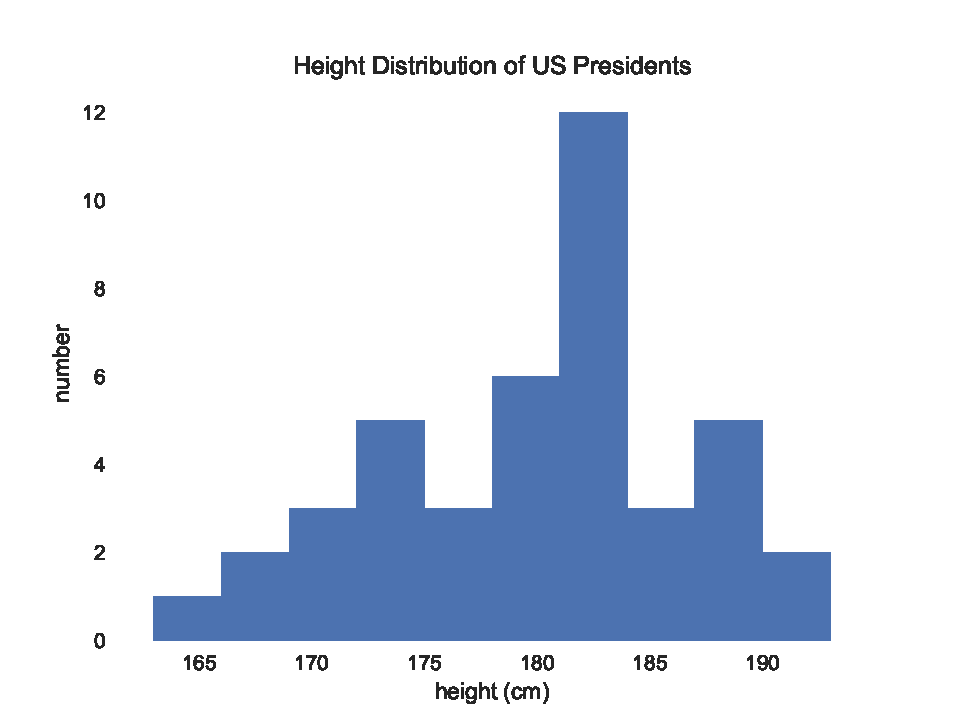
\includegraphics[width=0.4\textwidth]{figs/presidents.pdf}	
\end{frame}

\subsection{Broadcasting}
\begin{frame}[fragile]{Universal functions}{Broadcasting (I)}
	Broadcasting is a mechanism to operate over arrays of different sizes
	\begin{itemize}
		\item Used in ufuncs
		\item Implicit array expansion through three rules
	\end{itemize}
	\vspace{-0.2cm} 
	\begin{columns}
 	   \column{0.9\textwidth}
		\begin{block}{\footnotesize{Broadcasting rules}}
		\vspace{-0.2cm} 
		\begin{enumerate}
		\item Rule 1: If the two arrays differ in their number of dimensions, the shape of the one with fewer dimensions is padded with ones on its leading (left) side.
		\item Rule 2: If the shape of the two arrays does not match in any dimension, the array with shape equal to 1 in that dimension is stretched to match the other shape.
		\item Rule 3: If in any dimension the sizes disagree and neither is equal to 1, an error is raised.
		\end{enumerate}
		\vspace{-0.2cm} 
		\end{block}
	\end{columns}
\end{frame}

\begin{frame}[fragile]{Universal functions}{Broadcasting (II)}
	\vspace{-0.2cm} 
	\begin{columns}
 	   \column{0.7\textwidth}
		\centering 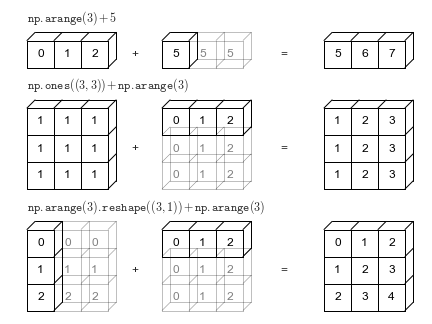
\includegraphics[width=\textwidth]{figs/02.05-broadcasting.png}	
 	   \column{0.3\textwidth}
	   	Array expansion does not consume memory!
	\end{columns}
\end{frame}

\begin{frame}[fragile]{Universal functions}{Broadcasting (III)}
	\vspace{-0.2cm} 
	\begin{columns}
 	   \column{0.7\textwidth}
		\begin{exampleblock}{Normalization}
		\vspace{-0.2cm} 
			\begin{lstlisting}
			X = np.random.random((10, 3))
			Xmean = X.mean(0)
			X_centered = X - Xmean
			\end{lstlisting}
		\vspace{-0.2cm} 
		\end{exampleblock}

		\begin{exampleblock}{3D plot}
		\vspace{-0.2cm} 
			\begin{lstlisting}[language=Python]
			%matplotlib inline
			import matplotlib.pyplot as plt

			x = np.linspace(0, 5, 50)
			y = np.linspace(0, 5, 50)[:, np.newaxis]
			z = np.sin(x)**10+np.cos(10+y*x)*np.cos(x)

			plt.imshow(z, origin='lower', 
			    extent=[0, 5, 0, 5], cmap='viridis')
			plt.colorbar();
			\end{lstlisting}
		\vspace{-0.2cm} 
		\end{exampleblock}

 	   \column{0.3\textwidth}
			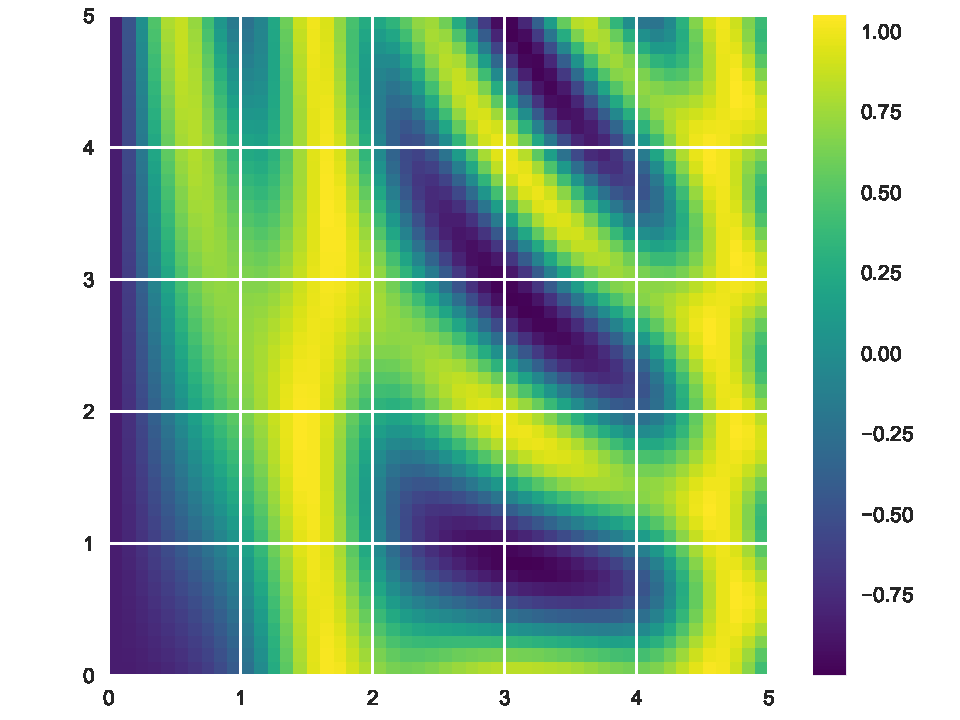
\includegraphics[width=\textwidth]{figs/3dplot.pdf}	
	\end{columns}
\end{frame}

\section{Comparisons, masks and Boolean logic}
\subsection{Motivation}

\begin{frame}[fragile]{Comparisons, masks and Boolean logic}{Motivation (I)}
	\vspace{-0.2cm} 
	\begin{columns}
 	   \column{0.9\textwidth}
		\href{https://raw.githubusercontent.com/jakevdp/PythonDataScienceHandbook/master/notebooks/data/Seattle2014.csv}{(Download dataset)}
		\begin{exampleblock}{Example}
		\vspace{-0.2cm} 
			\begin{lstlisting}
			import numpy as np
			import pandas as pd
             
			# pandas to extract rainfall inches as a ndarray
			rainfall = pd.read_csv('Seattle2014.csv')['PRCP'].values
			inches = rainfall / 254.0  # 1/10mm -> inches
			inches.shape 
			# Outputs (365,)
			 
			%matplotlib 
			import matplotlib.pyplot as plt
			import seaborn; seaborn.set()
			plt.hist(inches, 40);
			\end{lstlisting}
		\vspace{-0.2cm} 
		\end{exampleblock}
	\end{columns}
\end{frame}

\begin{frame}[fragile]{Comparisons, masks and Boolean logic}{Motivation (II)}
	\begin{columns}
 	   \column{0.4\textwidth}
		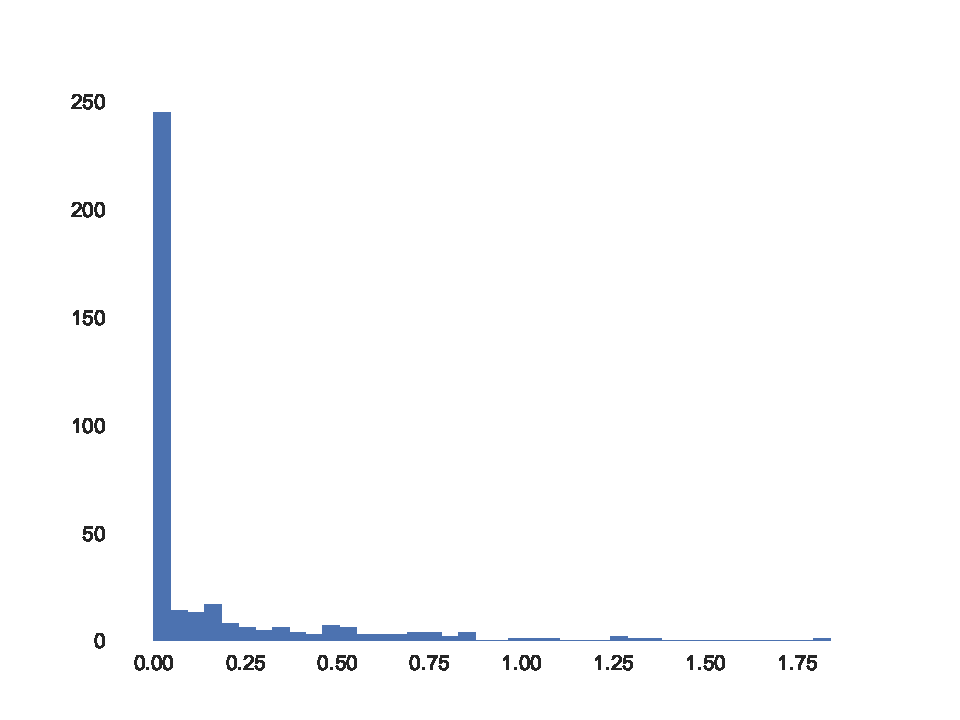
\includegraphics[width=\textwidth]{figs/rain.pdf}	
	\end{columns}

	Data filtering is a recurrent task
	\begin{itemize}
		\item How many rainy days were there in the year?
		\item What is the average precipitation on those rainy days?
		\item How many days were there with more than half an inch of rain?
	\end{itemize}

	Two filtering methods in NumPy
	\begin{itemize}
		\item Boolean arrays masks
		\item Fancy indexing
	\end{itemize}
\end{frame}

\begin{frame}[fragile]{Comparisons, masks and Boolean logic}{Boolean arrays masks (I)}
	\begin{columns}
 	   \column{0.3\textwidth}
		\begin{exampleblock}{\footnotesize{Syntax examples}}
		\vspace{-0.2cm} 
			\begin{lstlisting}
				x[x<5]
				x[x==3]
				x[(x>3)&(x<=5)]
			\end{lstlisting}
		\vspace{-0.2cm} 
		\end{exampleblock}
	\end{columns}

	\bigskip

	We've seen arithmetic ufuncs ...
	\begin{itemize}
		\item ... but they also support comparison and boolean operations
		\item Return an array of booleans
	\end{itemize}

	\footnotesize{
	\begin{columns}
 	   \column{0.5\textwidth}
       \begin{tabular}{ll}\hline
       	\textsc{Operator} &  \textsc{Ufunc}\\ \hline
       	== & \texttt{np.equal}  \\
       	!= & \texttt{np.not\_equal}  \\
       	<  & \texttt{np.less}  \\
       	<= & \texttt{np.less\_equal}  \\
       	>  & \texttt{np.greater}  \\
       	>= & \texttt{np.greater\_equal}\\\hline
    	\end{tabular}

 	   \column{0.5\textwidth}
        \begin{tabular}{ll}\hline
       	\textsc{Operator} &  \textsc{Ufunc}\\ \hline
       	\& & \texttt{np.bitwise\_and} \\
       	|  & \texttt{np.bitwise\_or}  \\
       	\textasciicircum & \texttt{np.bitwise\_xor} \\
       	\textasciitilde & \texttt{np.bitwise\_not} \\\hline
    	\end{tabular}
	\end{columns}
	}
\end{frame}

\begin{frame}[fragile]{Comparisons, masks and Boolean logic}{Boolean arrays masks (II)}
	\begin{columns}
 	   \column{0.7\textwidth}
		\begin{exampleblock}{\footnotesize{Example}}
		\vspace{-0.2cm} 
			\begin{lstlisting}
				print(x)
				[[5, 0, 3, 3]
				 [7, 9, 3, 5]
				 [2, 4, 7, 6]]
				np.count_nonzero(x < 6) # Returns 8
				np.sum(x < 6) # Returns 8
				np.sum(x < 6, axis=1) # By row, returns array([4,2,2])
				np.any(x > 8) # Returns True
				np.any(x < 0) # Returns False
				np.all(x < 10)# Returns True

				np.sum(~((inches <= 5) | (inches >= 1)))
			\end{lstlisting}
		\vspace{-0.2cm} 
		\end{exampleblock}
	\end{columns}
\end{frame}

\begin{frame}[fragile]{Comparisons, masks and Boolean logic}{Fancy indexing}
	\begin{columns}
 	   \column{0.4\textwidth}
	So far we've seen three accessing methods
	\begin{itemize}
		\item Simple indices (\texttt{x[1]})
		\item Slices (\texttt{x[:5]})
		\item Boolean masks (\texttt{x[x>0]})
	\end{itemize}
	Fancy indexing: Pass arrays on indices instead of scalars
 	   \column{0.6\textwidth}
		\begin{exampleblock}{\footnotesize{Example}}
		\vspace{-0.2cm} 
			\begin{lstlisting}
				x = rand.randint(100, size=10)
				[x[3], x[7], x[2]] # Simple indices
				ind = [3, 7, 4] # Array of indices
				x[ind] # Fancy indexing
				x[[3,5,6]] # Also valid
			\end{lstlisting}
		\vspace{-0.2cm} 
		\end{exampleblock}

		\footnotesize{
		\begin{alertblock}{}
		The shape of the result reflects the shape of the index arrays rather than the shape of the array being indexed
		\end{alertblock}
		}
	\end{columns}
\end{frame}

\section{Structured arrays}

\begin{frame}[fragile]{Structured arrays (I)}
	Some times, we need to group data
	\begin{itemize}
		\item Example: Store name, age and weight of several people
		\item Different data types for each attribute
	\end{itemize}
	\begin{columns}
 	   \column{\textwidth}
		\begin{exampleblock}{\footnotesize{Non-structured array}}
		\vspace{-0.2cm} 
		\begin{lstlisting}
			name = ['Alice', 'Bob', 'Cathy', 'Doug']
			age = [25, 45, 37, 19]
			weight = [55.0, 85.5, 68.0, 61.5]
		\end{lstlisting}
		\vspace{-0.2cm} 
	\end{exampleblock}
	
	\vspace{-0.2cm}
	\begin{flushleft}
	Solution: Structured arrays
	\end{flushleft}
	\vspace{-0.2cm}
	\begin{exampleblock}{\footnotesize{Structured arrays}}
		\vspace{-0.2cm} 
		\begin{lstlisting}
		# Use a compound data type for structured arrays
		data = np.zeros(4, dtype={'names':('name', 'age', 'weight'),
                          'formats':('U10', 'i4', 'f8')})
		\end{lstlisting}
		\vspace{-0.2cm} 
	\end{exampleblock}
	\end{columns}
\end{frame}

\begin{frame}[fragile]{Structured arrays (II)}
	\begin{columns}
 	   \column{0.6\textwidth}
	\begin{exampleblock}{\footnotesize{Structured array manipulation}}
		\vspace{-0.2cm} 
		\begin{lstlisting}
		data['name'] = name
		data['age'] = age
		data['weight'] = weight

		# Get all names
		data['name']
		# Get first row of data
		data[0]
		# Get the name from the last row
		data[-1]['name']
		# Get names where age is under 30
		data[data['age'] < 30]['name']
		\end{lstlisting}
		\vspace{-0.2cm} 
	\end{exampleblock}

	\bigskip

	\end{columns}
	These kind of structures are day-to-day used
	\begin{itemize}
		\item Pandas is a much better choice
	\end{itemize}
\end{frame}

\end{document}
